\section{Model Fitting and Line and Circle Detection}

Edge detection alone is often insufficient, as images may contain multiple lines and numerous edges unrelated to lines.
Noise in line edges can cause misalignment, and lines may not be complete.

\subsection{Model Fitting}

Model fitting is an algorithm that identifies a high-level model to explain observations effectively.
Here, edges serve as observations, and the model consists of one or more lines.

\subsection{Voting Algorithms}

Voting algorithms are a general technique for decision methods.

\begin{enumerate}
	\item Every feature casts votes for all compatible models.
	\item Models accumulating many votes are chosen.
\end{enumerate}

Clutter and noise may cast many votes but lack consistency. Features belonging to a model concentrate votes for that model.

\subsection{Hough Transform}

\begin{enumerate}
	\item Every \textbf{edge point} casts votes for \textbf{all compatible lines}.
	\item \textbf{Lines} accumulating many votes are chosen.
\end{enumerate}

\begin{figure}[H]
	\centering
	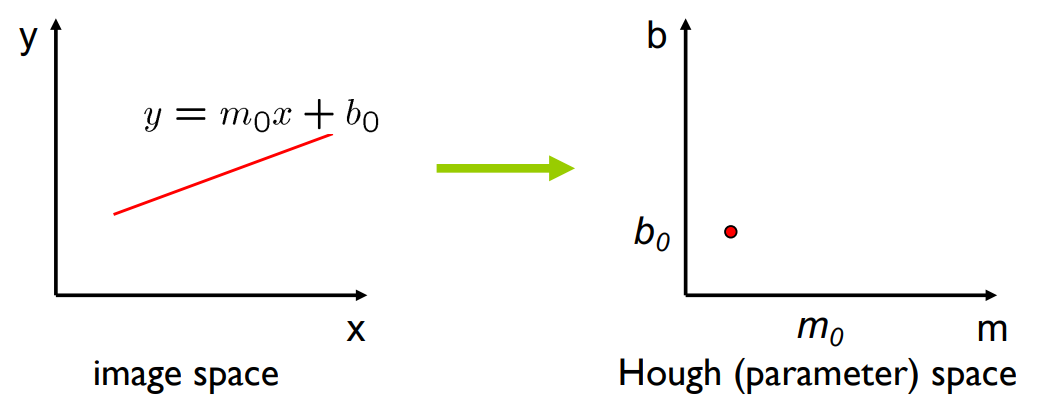
\includegraphics[width=0.7\linewidth,keepaspectratio]{img/line_representation_hough}
	\caption{Line representation in Hough space}
\end{figure}

\begin{figure}[H]
	\centering
	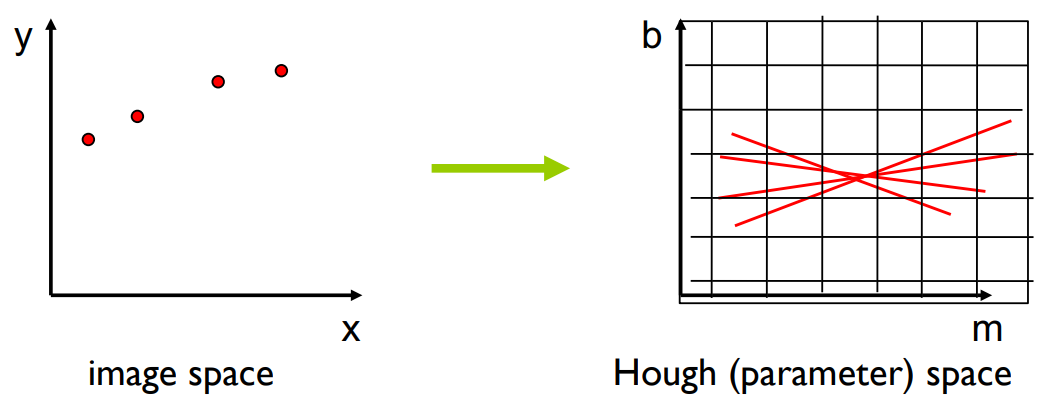
\includegraphics[width=0.7\linewidth]{img/points_representation_hough}
	\caption{Points on a line in normal space almost intersect in Hough space}
	\label{fig:pointsrepresentationhough}
\end{figure}

The problem with this approach is that
\begin{enumerate}[label=\alph*.]
	\item the parameter space $(m,b)$ is \textbf{not bounded}
	\item \textbf{vertical lines} cannot be represented
\end{enumerate}

\subsection{Representation of Lines in Polar Coordinates}

\begin{figure}[H]
	\centering
	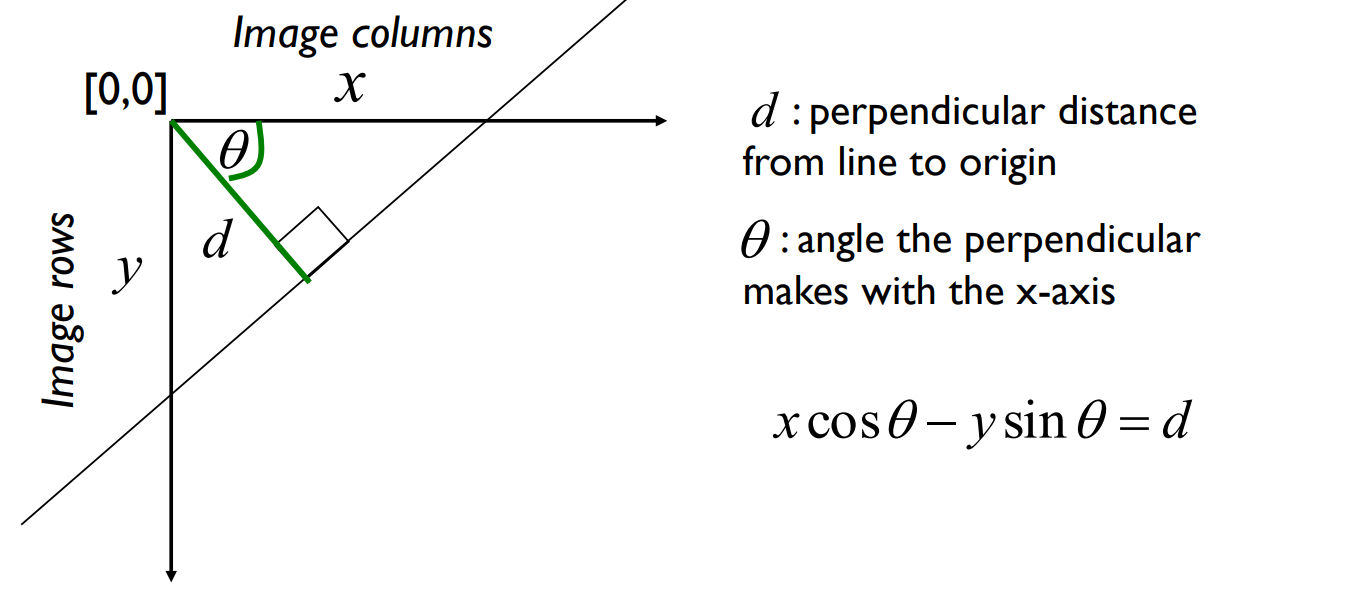
\includegraphics[width=0.7\linewidth]{img/line_representation_polar}
	\caption{Line representation with polar parameters}
	\label{fig:linerepresentationpolar}
\end{figure}

This approach solves both the problems of unboundedness and representation. The parameters $\theta$ and $d$ have bounded ranges.

For every point in normal space, there will be a sinusoid in the polar Hough space.

\subsection{Hough Transformation Algorithm}

The algorithm transforms each edge point in the image to Hough space, where an Accumulator array gets filled with votes.
The bin size of the accumulator is an important hyperparameter. If too small, there will be many weak peaks due to noise;
if too large, accuracy of locating a line drops, and clutter votes might end up in the same bin.
A solution is to keep the bin size small but also count votes from neighbors.

\subsubsection{Voting Algorithm for Finding Lines}

\begin{enumerate}
	\item Every edge point casts votes for all circles that are compatible with it.
	\item Circles accumulating many votes are chosen.
\end{enumerate}

\begin{theorem}
	Parametrization of a circle:
	\begin{equation*}
		(x_i - a)^2 + (y_i - b)^2 = r^2
	\end{equation*}
	With center $(a,b)$ and radius $r$.
\end{theorem}

\begin{center}
	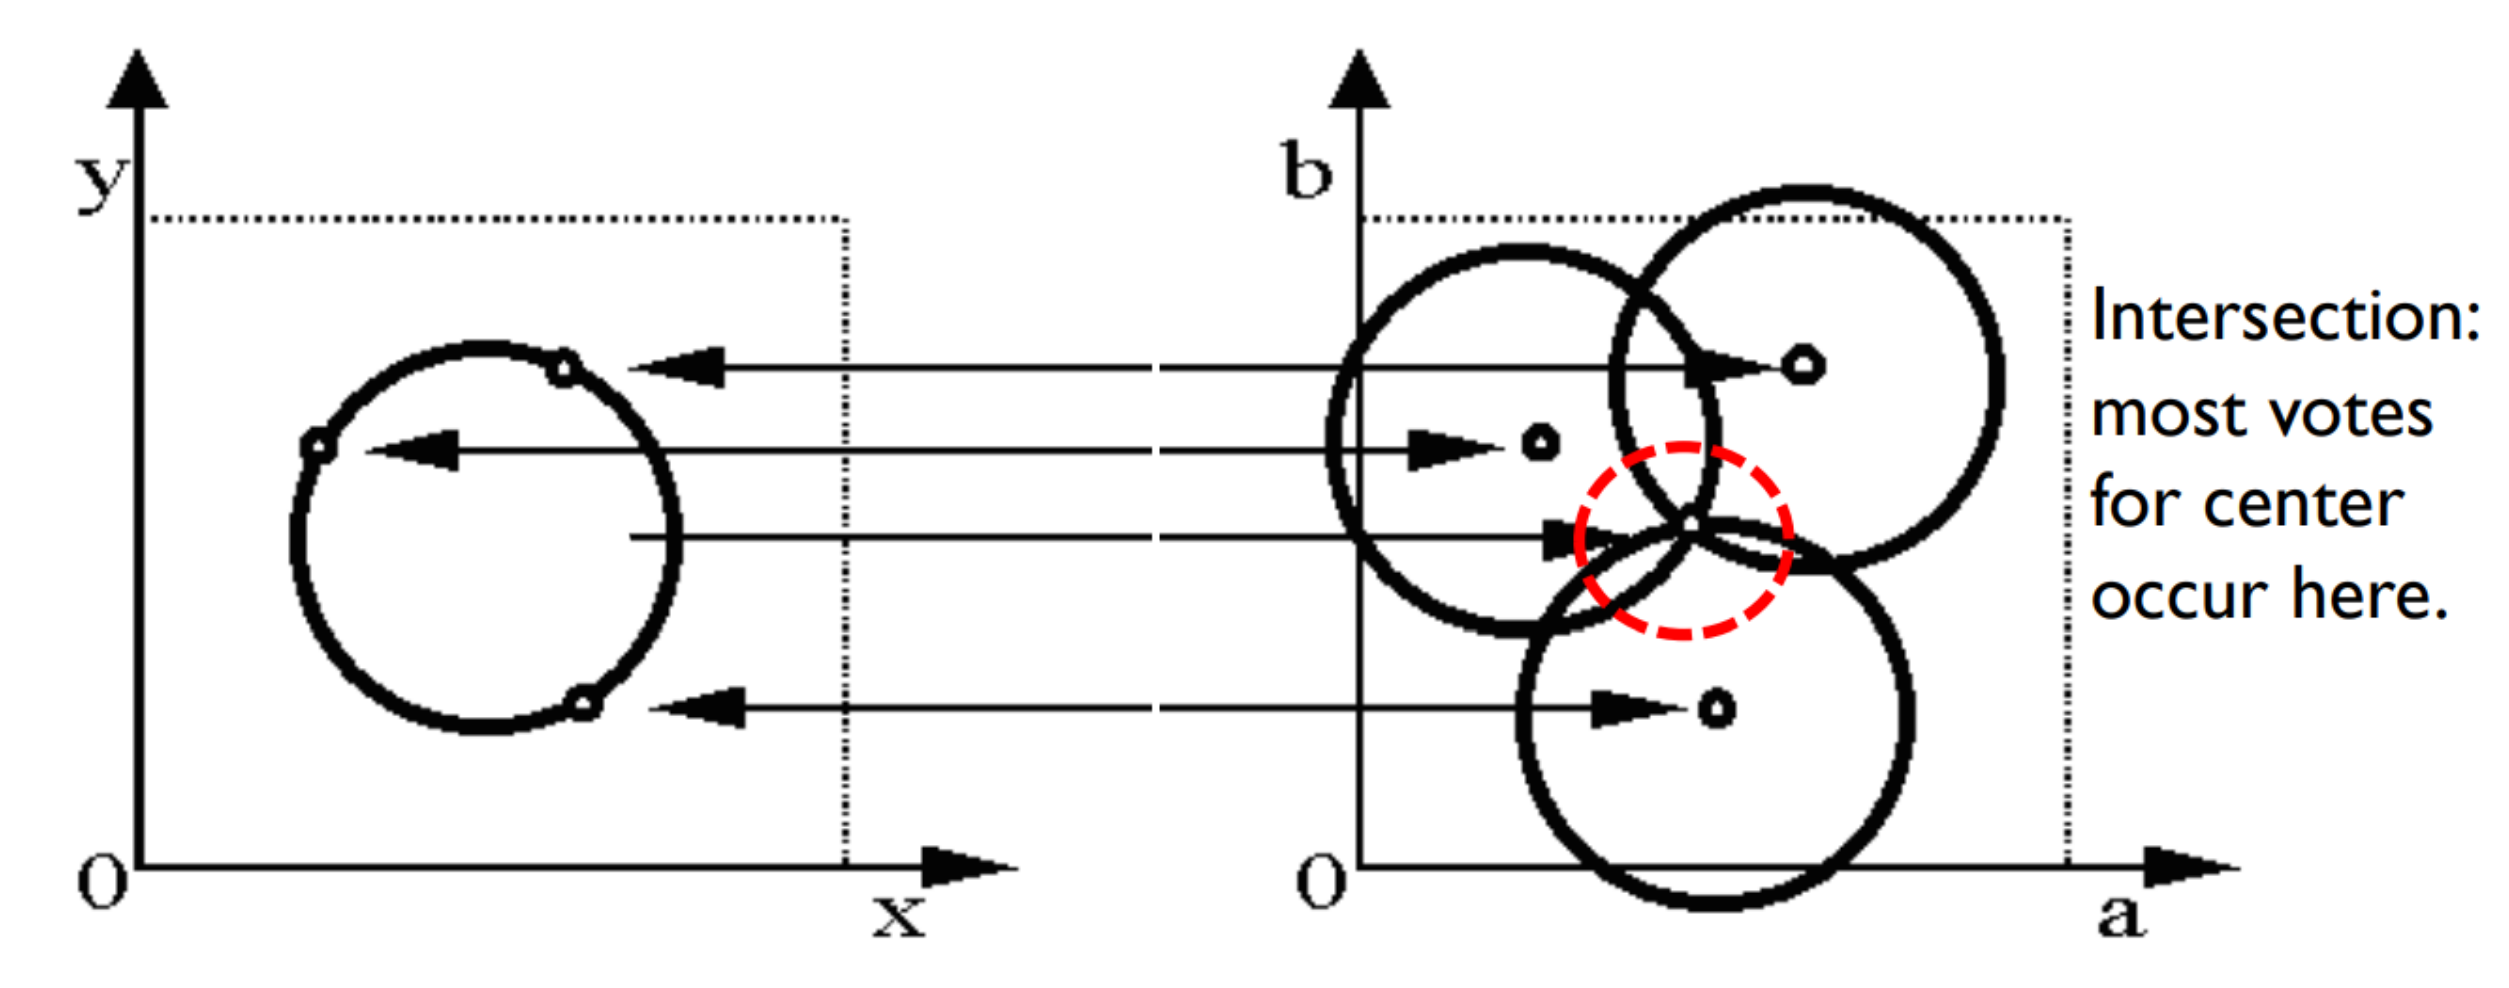
\includegraphics[width=0.7\linewidth]{img/hough_circle_accumulator}
\end{center}

\subsection{Hough Space for Circles With Unknown Radius}

\begin{center}
	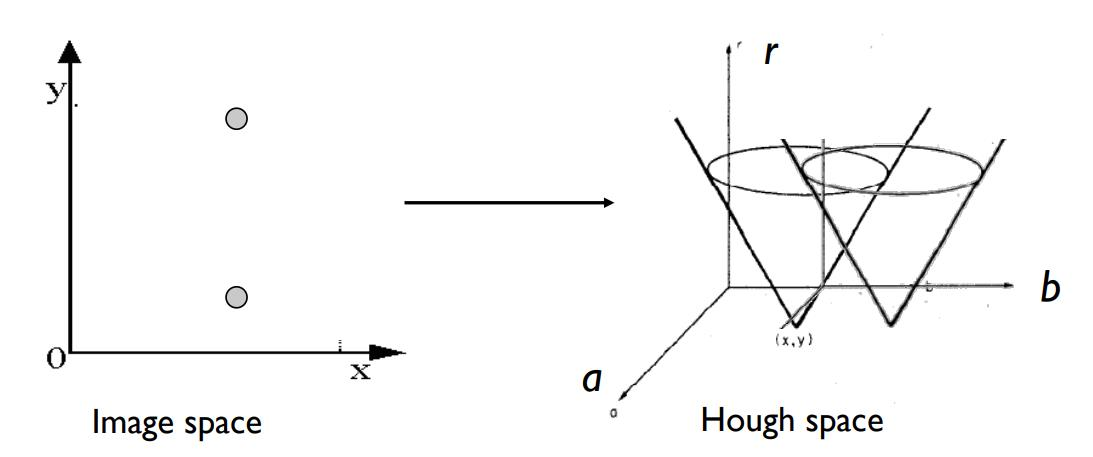
\includegraphics[width=0.7\linewidth]{img/hough_circle_accumulator_point}
\end{center}

\begin{equation*}
	y = a\cdot x + \sout{b}
\end{equation*}
